\section{H2}
\subsection*{Material ID: mp-bgmia}
\textbf{Constante Dieléctrica ($\epsilon_{total}$):} 1.25 \\[0.5em]
\begin{table}[h!]
\centering
\begin{tabular}{lcc}
\toprule
\textbf{Métrica} & \textbf{Lámina (Plate)} & \textbf{Cilindros (Rod)} \\
\midrule
Bandgaps ($a/\lambda$) & Ninguno & Ninguno \\
Resonancias & 36 & 36 \\
\bottomrule
\end{tabular}
\end{table}
\begin{figure}[H]
\centering
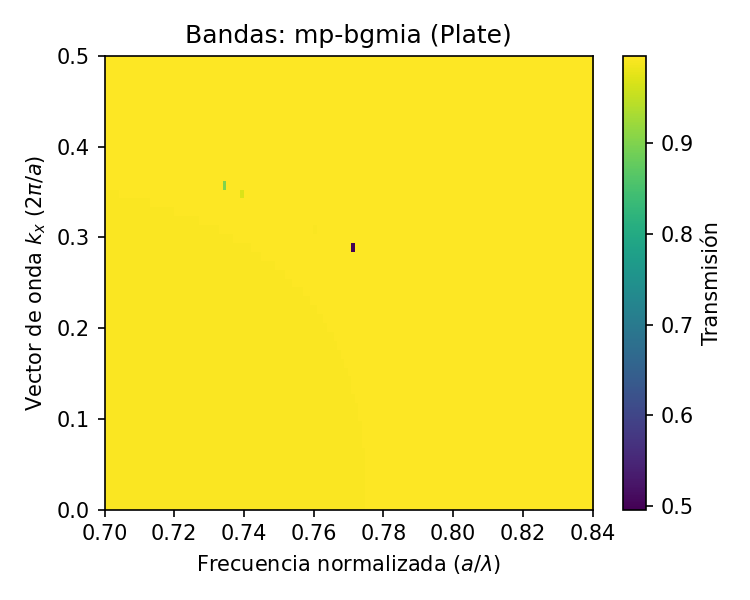
\includegraphics[width=0.48\textwidth]{figures/mp-bgmia_plate.png}
\hfill
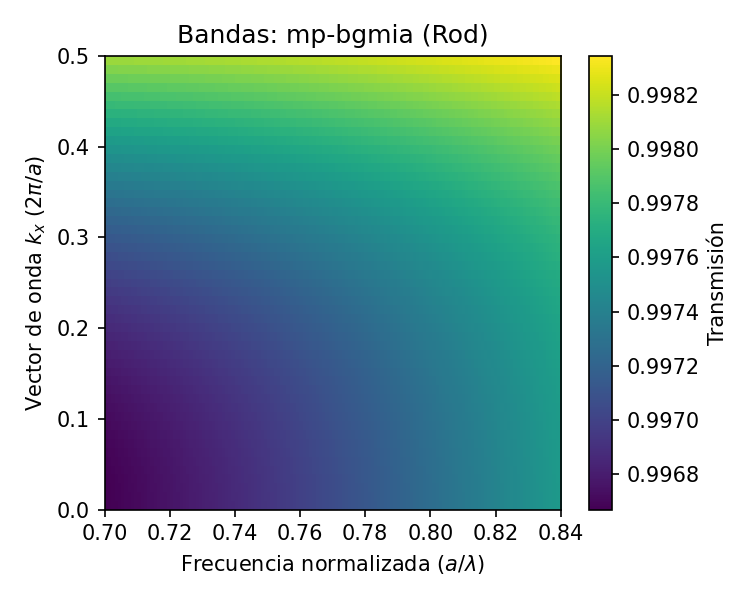
\includegraphics[width=0.48\textwidth]{figures/mp-bgmia_rod.png}
\caption{Estructuras de bandas fotónicas para mp-bgmia. Izquierda: Lámina. Derecha: Cilindros.}
\end{figure}
\vspace{1em}
\hrule
\vspace{1em}
\subsection*{Material ID: mp-bjjn}
\textbf{Constante Dieléctrica ($\epsilon_{total}$):} 1.26 \\[0.5em]
\begin{table}[h!]
\centering
\begin{tabular}{lcc}
\toprule
\textbf{Métrica} & \textbf{Lámina (Plate)} & \textbf{Cilindros (Rod)} \\
\midrule
Bandgaps ($a/\lambda$) & Ninguno & Ninguno \\
Resonancias & 36 & 36 \\
\bottomrule
\end{tabular}
\end{table}
\begin{figure}[H]
\centering
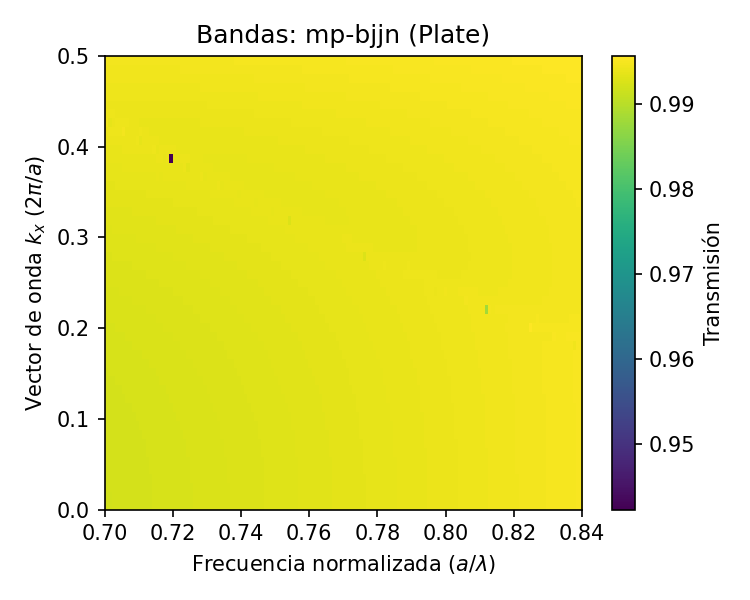
\includegraphics[width=0.48\textwidth]{figures/mp-bjjn_plate.png}
\hfill
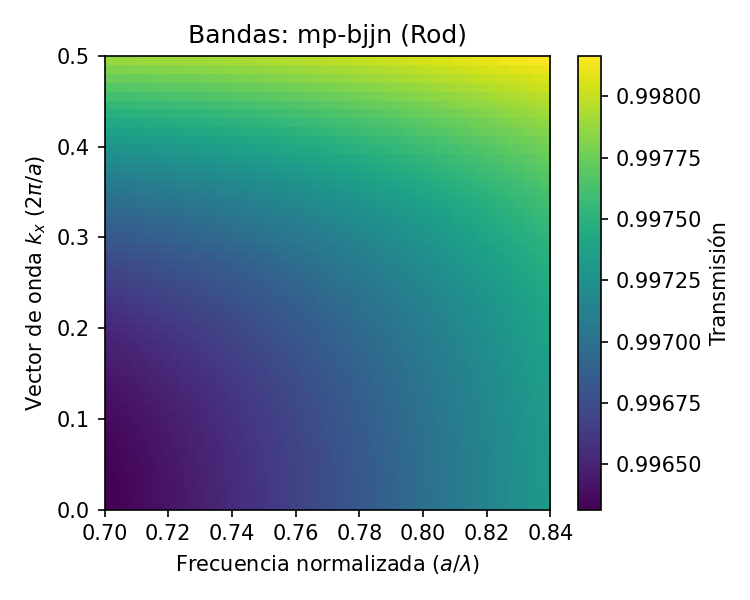
\includegraphics[width=0.48\textwidth]{figures/mp-bjjn_rod.png}
\caption{Estructuras de bandas fotónicas para mp-bjjn. Izquierda: Lámina. Derecha: Cilindros.}
\end{figure}
\vspace{1em}
\hrule
\vspace{1em}
\subsection*{Material ID: mp-bjzhi}
\textbf{Constante Dieléctrica ($\epsilon_{total}$):} 1.16 \\[0.5em]
\begin{table}[h!]
\centering
\begin{tabular}{lcc}
\toprule
\textbf{Métrica} & \textbf{Lámina (Plate)} & \textbf{Cilindros (Rod)} \\
\midrule
Bandgaps ($a/\lambda$) & Ninguno & Ninguno \\
Resonancias & 36 & 36 \\
\bottomrule
\end{tabular}
\end{table}
\begin{figure}[H]
\centering
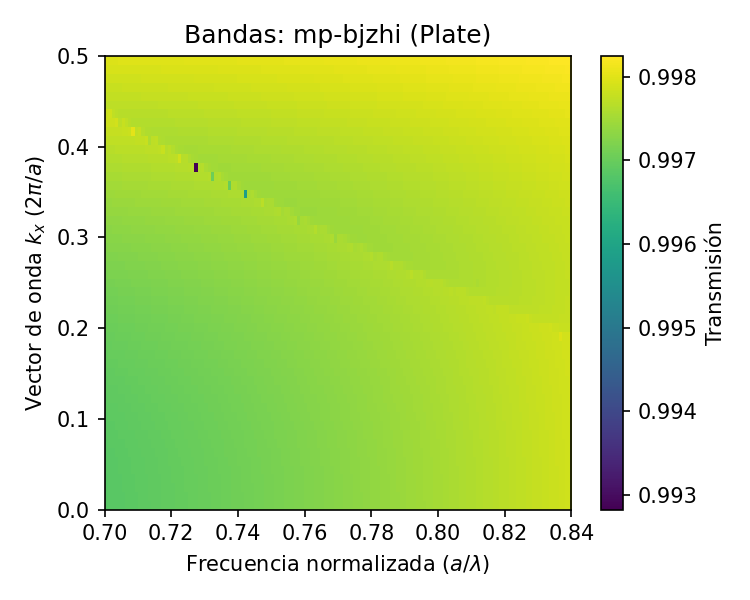
\includegraphics[width=0.48\textwidth]{figures/mp-bjzhi_plate.png}
\hfill
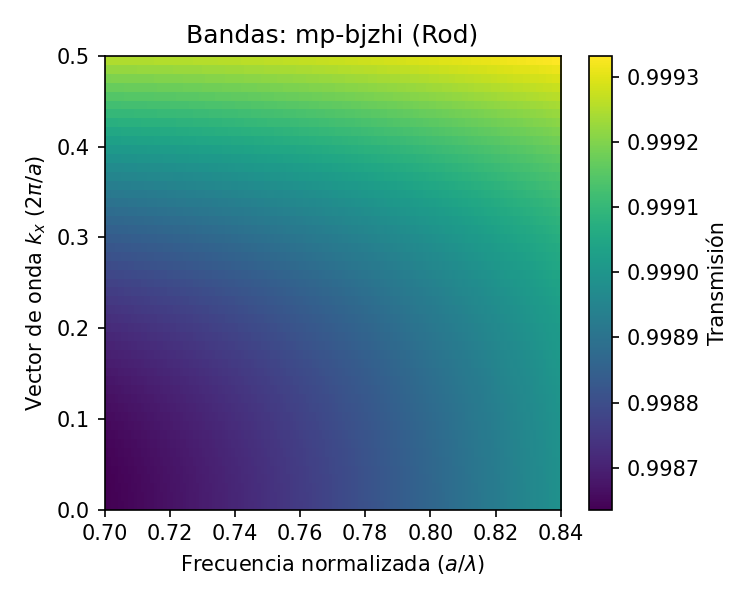
\includegraphics[width=0.48\textwidth]{figures/mp-bjzhi_rod.png}
\caption{Estructuras de bandas fotónicas para mp-bjzhi. Izquierda: Lámina. Derecha: Cilindros.}
\end{figure}
\vspace{1em}
\hrule
\vspace{1em}
\subsection*{Material ID: mp-bjzix}
\textbf{Constante Dieléctrica ($\epsilon_{total}$):} 1.53 \\[0.5em]
\begin{table}[h!]
\centering
\begin{tabular}{lcc}
\toprule
\textbf{Métrica} & \textbf{Lámina (Plate)} & \textbf{Cilindros (Rod)} \\
\midrule
Bandgaps ($a/\lambda$) & Ninguno & Ninguno \\
Resonancias & 36 & 36 \\
\bottomrule
\end{tabular}
\end{table}
\begin{figure}[H]
\centering
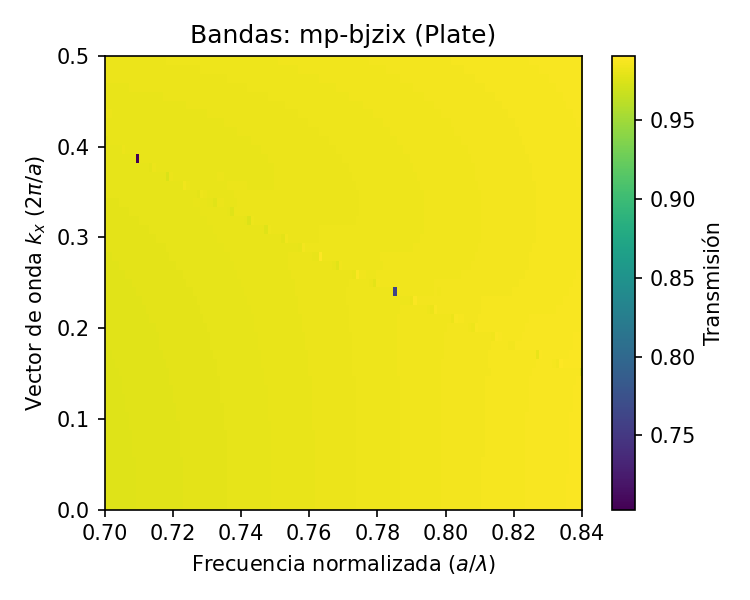
\includegraphics[width=0.48\textwidth]{figures/mp-bjzix_plate.png}
\hfill
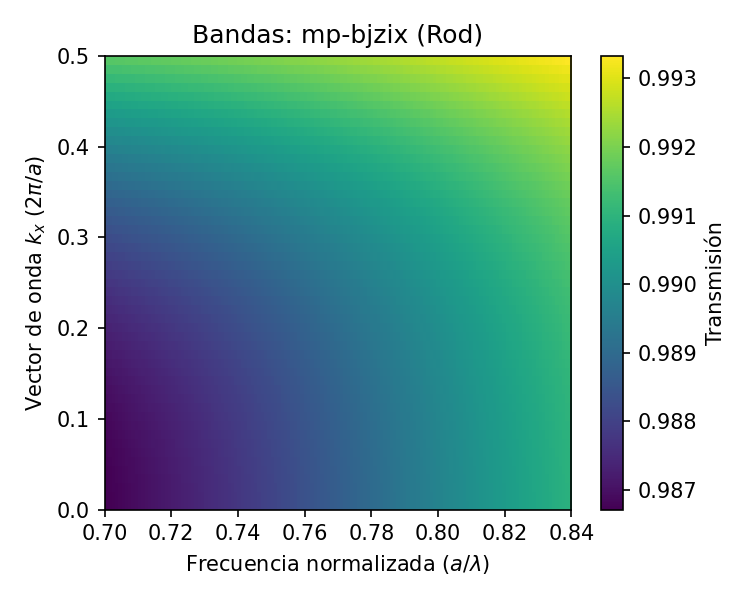
\includegraphics[width=0.48\textwidth]{figures/mp-bjzix_rod.png}
\caption{Estructuras de bandas fotónicas para mp-bjzix. Izquierda: Lámina. Derecha: Cilindros.}
\end{figure}
\vspace{1em}
\hrule
\vspace{1em}
\subsection*{Material ID: mp-bwjuw}
\textbf{Constante Dieléctrica ($\epsilon_{total}$):} 1.55 \\[0.5em]
\begin{table}[h!]
\centering
\begin{tabular}{lcc}
\toprule
\textbf{Métrica} & \textbf{Lámina (Plate)} & \textbf{Cilindros (Rod)} \\
\midrule
Bandgaps ($a/\lambda$) & Ninguno & Ninguno \\
Resonancias & 36 & 36 \\
\bottomrule
\end{tabular}
\end{table}
\begin{figure}[H]
\centering
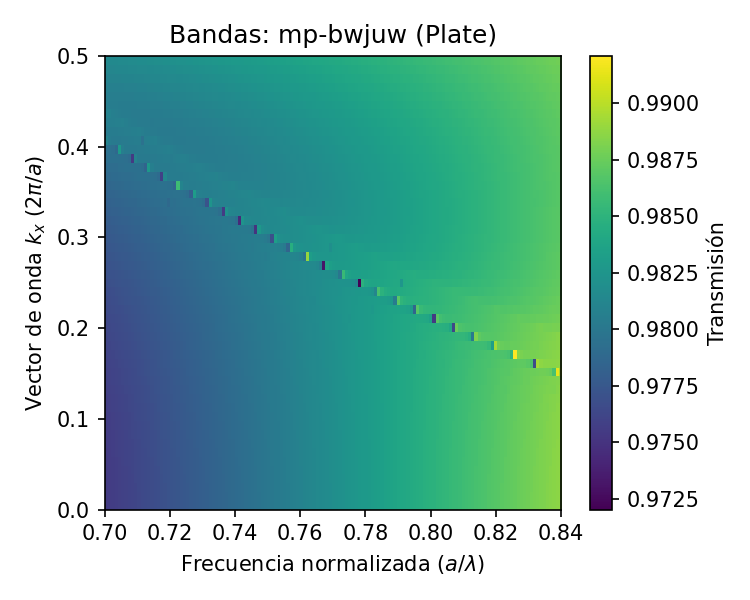
\includegraphics[width=0.48\textwidth]{figures/mp-bwjuw_plate.png}
\hfill
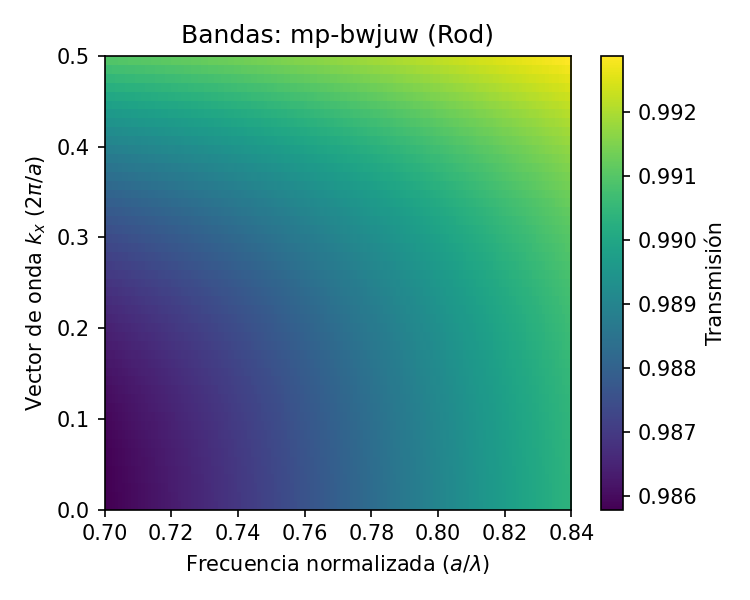
\includegraphics[width=0.48\textwidth]{figures/mp-bwjuw_rod.png}
\caption{Estructuras de bandas fotónicas para mp-bwjuw. Izquierda: Lámina. Derecha: Cilindros.}
\end{figure}
\vspace{1em}
\hrule
\vspace{1em}
\clearpage